\documentclass[uplatex]{jsarticle}

\usepackage{float}
\usepackage[dvipdfmx]{hyperref, graphicx}
\usepackage{pxjahyper}
\hypersetup{
	colorlinks=false, % リンクに色をつけない設定
	bookmarks=true, % 以下ブックマークに関する設定
	bookmarksnumbered=true,
	pdfborder={0 0 0},
	bookmarkstype=toc,
}
\newcommand{\linedhref}[2]{\underline{\href{#1}{\emph{#2}}}}

\begin{document}

吾輩は猫である。名前はまだ無い\cite{Soseki1905}。

どこで生れたかとんと見当がつかぬ。
何でも薄暗いじめじめした所で
ニャーニャー泣いていた事だけは記憶している。
吾輩はここで始めて人間というものを見た。

\begin{figure}[H]
	\begin{center}
		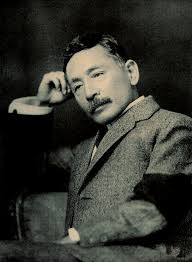
\includegraphics[height=10cm]{img/natsume_soseki.jpeg}
		\caption{夏目漱石の写真(引用元:\linedhref{https://ja.wikipedia.org/wiki/\%E5\%A4\%8F\%E7\%9B\%AE\%E6\%BC\%B1\%E7\%9F\%B3}{夏目漱石 - Wikipedia})}
	\end{center}
\end{figure}

\bibliography{ref}
\bibliographystyle{junsrt}

\end{document}